\chapter{Graphs and plots}
\label{chap:graphs}

\section{Gnuplot graphs}
\label{gnuplot-graphs}

A separate program, \app{gnuplot}, is called to generate graphs.
Gnuplot is a very full-featured graphing program with myriad options.
It is available from \href{http://www.gnuplot.info/}{www.gnuplot.info}
(but note that a suitable copy of gnuplot is bundled with the packaged
versions of gretl for MS Windows and Mac OS X).  Gretl gives you
direct access, via a graphical interface, to a subset of gnuplot's
options and it tries to choose sensible values for you; it also allows
you to take complete control over graph details if you wish.

With a graph displayed, you can click on the graph window for a pop-up
menu with the following options.

\begin{itemize}
\item \textsf{Save as PNG}: Save the graph in Portable Network
  Graphics format (the same format that you see on screen).
\item \textsf{Save as postscript}: Save in encapsulated postscript
  (EPS) format.
\item \textsf{Save as Windows metafile}: Save in Enhanced Metafile
  (EMF) format.
\item \textsf{Save to session as icon}: The graph will appear in
  iconic form when you select ``Icon view'' from the View menu.
\item \textsf{Zoom}: Lets you select an area within the graph for
  closer inspection (not available for all graphs).
\item \textsf{Print}: (Current GTK or MS Windows only) lets you
  print the graph directly.
\item \textsf{Copy to clipboard}: MS Windows only, lets you paste the
  graph into Windows applications such as MS Word.
\item \textsf{Edit}: Opens a controller for the plot which lets you
  adjust many aspects of its appearance.
\item \textsf{Close}: Closes the graph window.
\end{itemize}


\subsection{Displaying data labels}
\label{plot-labels}

For simple X-Y scatter plots, some further options are available if
the dataset includes ``case markers'' (that is, labels identifying
each observation).\footnote{For an example of such a dataset, see the
  Ramanathan file \verb+data4-10+: this contains data on private
  school enrollment for the 50 states of the USA plus Washington, DC;
  the case markers are the two-letter codes for the states.} With a
scatter plot displayed, when you move the mouse pointer over a data
point its label is shown on the graph.  By default these labels are
transient: they do not appear in the printed or copied version of the
graph.  They can be removed by selecting ``Clear data labels'' from
the graph pop-up menu. If you want the labels to be affixed
permanently (so they will show up when the graph is printed or
copied), select the option ``Freeze data labels'' from the pop-up
menu; ``Clear data labels'' cancels this operation.  The other
label-related option, ``All data labels'', requests that case markers
be shown for all observations.  At present the display of case markers
is disabled for graphs containing more than 250 data points.


\subsection{GUI plot editor}
\label{plot-editor}

Selecting the \textsf{Edit} option in the graph popup menu opens
an editing dialog box, shown in Figure~\ref{fig-plot}.  Notice that
there are several tabs, allowing you to adjust many aspects of
a graph's appearance: font, title, axis scaling, line colors
and types, and so on.  You can also add lines or descriptive
labels to a graph (under the Lines and Labels tabs).  The
``Apply'' button applies your changes without closing the
editor; ``OK'' applies the changes and closes the dialog.

\begin{figure}[htbp]
  \begin{center}
    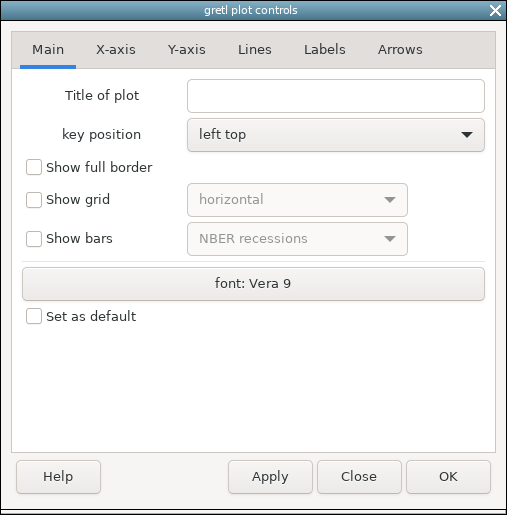
\includegraphics[scale=0.6]{figures/plot_control}
  \end{center}
  \caption{gretl's gnuplot controller}
  \label{fig-plot}
\end{figure}


\subsection{Publication-quality graphics: advanced options}
\label{plot-advanced}

The GUI plot editor has two limitations.  First, it cannot represent
all the myriad options that \app{gnuplot} offers. Users who are
sufficiently familiar with \app{gnuplot} to know what they're missing
in the plot editor presumably don't need much help from gretl,
so long as they can get hold of the \app{gnuplot} command file that
gretl has put together.  Second, even if the plot editor meets
your needs, in terms of fine-tuning the graph you see on screen, a few
details may need further work in order to get optimal results for
publication.

Either way, the first step in advanced tweaking of a graph is to get
access to the graph command file.

\begin{itemize}
\item In the graph display window, right-click and choose ``Save to
  session as icon''.
\item If it's not already open, open the icon view window---either
  via the menu item View/Icon view, or by clicking the ``session icon
  view'' button on the main-window toolbar.
\item Right-click on the icon representing the newly added graph and
  select ``Edit plot commands'' from the pop-up menu.
\item You get a window displaying the plot file
  (Figure~\ref{fig:plot-edit}).
\end{itemize}

\begin{figure}[htbp]
  \centering
  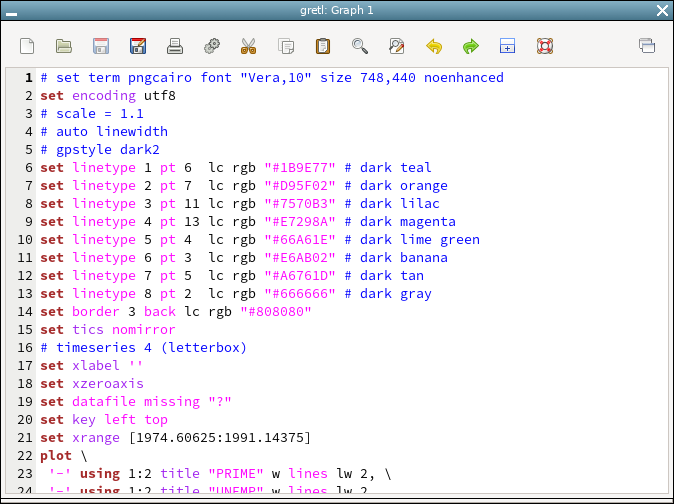
\includegraphics[scale=0.6]{figures/plotedit}
  \caption{Plot commands editor}
  \label{fig:plot-edit}
\end{figure}

Here are the basic things you can do in this window.  Obviously, you
can edit the file you just opened.  You can also send it for
processing by gnuplot, by clicking the ``Execute'' (cogwheel)
icon in the toolbar.  Or you can use the ``Save as'' button to save
a copy for editing and processing as you wish.

Unless you're a gnuplot expert, most likely you'll only need to edit a
couple of lines at the top of the file, specifying a driver (plus
options) and an output file.  We offer here a brief summary of some
points that may be useful.

First, \app{gnuplot}'s output mode is set via the command \texttt{set
  term} followed by the name of a supported driver (``terminal'' in
gnuplot parlance) plus various possible options.  (The top line in the
plot commands window shows the \texttt{set term} line that gretl
used to make a PNG file, commented out.)  The graphic formats that are
most suitable for publication are PDF and EPS.  These are supported by
the gnuplot \texttt{term} types \texttt{pdf}, \texttt{pdfcairo} and
\texttt{postscript} (with the \texttt{eps} option).  The
\texttt{pdfcairo} driver has the virtue that is behaves in a very
similar manner to the PNG one, the output of which you see on screen.
This is provided by the version of gnuplot that is included in the
gretl packages for MS Windows and Mac OS X; if you're on Linux
it may or may be supported.  If \texttt{pdfcairo} is not available,
the \texttt{pdf} terminal may be available; the \texttt{postscript}
terminal is almost certainly available.

Besides selecting a term type, if you want to get gnuplot to write the
actual output file you need to append a \texttt{set output} line
giving a filename.  Here are a few examples of the first two lines you
might type in the window editing your plot commands.  We'll make
these more ``realistic'' shortly.
%
\begin{code}
set term pdfcairo
set output 'mygraph.pdf'

set term pdf
set output 'mygraph.pdf'

set term postscript eps
set output 'mygraph.eps'
\end{code}

There are a couple of things worth remarking here.  First, you may
want to adjust the size of the graph, and second you may want to
change the font.  The default sizes produced by the above drivers are
5 inches by 3 inches for \texttt{pdfcairo} and \texttt{pdf}, and 5
inches by 3.5 inches for \texttt{postscript eps}.  In each case
you can change this by giving a size specification, which takes the
form \texttt{XX,YY} (examples below).  

You may ask, why bother changing the size in the gnuplot command file?
After all, PDF and EPS are both vector formats, so the graphs can be
scaled at will.  True, but a uniform scaling will also affect the font
size, which may end looking wrong.  You can get optimal results by
experimenting with the \texttt{font} and \texttt{size} options to
\app{gnuplot}'s \texttt{set term} command.  Here are some examples
(comments follow below).
%
\begin{code}
# pdfcairo, regular size, slightly amended
set term pdfcairo font "Sans,6" size 5in,3.5in
# or small size
set term pdfcairo font "Sans,5" size 3in,2in

# pdf, regular size, slightly amended
set term pdf font "Helvetica,8" size 5in,3.5in
# or small
set term pdf font "Helvetica,6" size 3in,2in

# postscript, regular 
set term post eps solid font "Helvetica,16"
# or small
set term post eps solid font "Helvetica,12" size 3in,2in
\end{code}

On the first line we set a sans serif font for \texttt{pdfcairo} at a
suitable size for a 5 $\times$ 3.5 inch plot (which you may find looks
better than the rather ``letterboxy'' default of 5 $\times$ 3).  And
on the second we illustrate what you might do to get a smaller 3
$\times$ 2 inch plot. You can specify the plot size in centimeters
if you prefer, as in
\begin{code}
set term pdfcairo font "Sans,6" size 6cm,4cm
\end{code}

We then repeat the exercise for the \texttt{pdf} terminal.  Notice
that here we're specifying one of the 35 standard PostScript fonts,
namely Helvetica.  Unlike \texttt{pdfcairo}, the plain \texttt{pdf}
driver is unlikely to be able to find fonts other than these.

In the third pair of lines we illustrate options for the
\texttt{postscript} driver (which, as you see, can be abbreviated as
\texttt{post}).  Note that here we have added the option
\texttt{solid}.  Unlike most other drivers, this one uses dashed lines
unless you specify the \texttt{solid} option.  Also note that we've
(apparently) specified a much larger font in this case.  That's
because the \texttt{eps} option in effect tells the
\texttt{postscript} driver to work at half-size (among other things),
so we need to double the font size.

Table~\ref{tab:drivers} summarizes the basics for the three drivers we
have mentioned.

\begin{table}[htbp]
  \centering
  \begin{tabular}{lcc}
    Terminal & default size (inches) & suggested font \\ [6pt]
    \texttt{pdfcairo} & 5 $\times$ 3 &   Sans,6 \\
    \texttt{pdf}      & 5 $\times$ 3 &   Helvetica,8 \\
    \texttt{post eps} & 5 $\times$ 3.5 & Helvetica,16 \\
  \end{tabular}
  \caption{Drivers for publication-quality graphics}
  \label{tab:drivers}
\end{table}

To find out more about \app{gnuplot} visit
\href{http://www.gnuplot.info/}{www.gnuplot.info}. This site has
documentation for the current version of the program in various
formats.

\subsection{Additional tips}
\label{subsect-graph-tips}

To be written.  Line widths, enhanced text.  Show a ``before and
after'' example.  

\section{Plotting graphs from scripts}
\label{sec:plotenv}

When working with scripts, you may want to have a graph shown onto
your display or saved into a file. In fact, if in your usual workflow
you find yourself creating similar graphs over and over again, you
might want to consider the option of writing a script which automates
this process for you. gretl gives you two main tools for doing
this: one is a command called \cmd{gnuplot}, whose main use is to
create standard plot quickly. The other one is the \cmd{plot} command
block, which has a more elaborate syntax but offers you more control
on output.

\subsection{The \cmd{gnuplot} command}
\label{sec:gnuplot-cmd}

The \cmd{gnuplot} command is described at length in the \GCR\ and the
online help system. Here, we just summarize its main features:
basically, it consists of the \cmd{gnuplot} keyword, followed by a
list of items, telling the command \emph{what} you want plotted and a
list of options, telling it \emph{how} you want it plotted.

For example, the line
\begin{code}
gnuplot y1 y2 x   
\end{code}
will give you a basic XY plot of the two series \texttt{y1} and
\texttt{y2} on the vertical axis versus the series \texttt{x} on the
horizontal axis. In general, the arguments to the \cmd{gnuplot}
command is a list of series, the last of which goes on the x-axis,
while all the other ones go onto the y-axis. By default, the
\cmd{gnuplot} command gives you a scatterplot. If you just have one
variable on the y-axis, then gretl will also draw a the OLS
interpolation, if the fit is good enough.\footnote{The technical
  condition for this is that the two-tailed $p$-value for the slope
  coefficient should be under 10\%.}

Several aspects of the behavior described above can be modified. You
do this by appending options to the command. Most options can be
broadly grouped in three categories:
\begin{enumerate}
\item Plot styles: we support points (the default choice), lines,
  lines and points together, and impulses (vertical lines). 
\item Algorithm for the fitted line: here you can choose between
  linear, quadratic and cubic interpolation, but also more exotic
  choices, such as semi-log, inverse or loess (non-parametric). Of
  course, you can also turn this feature off.
\item Input and output: you can choose whether you want your graph on
  your computer screen (and possibly use the in-built graphical widget
  to further customize it --- see above, page \pageref{plot-editor}),
  or rather save it to a file. We support several graphical formats,
  among which PNG and PDF, to make it easy to incorporate your
  plots into text documents.
\end{enumerate}

The following script uses the AWM dataset to exemplify some
traditional plots in macroeconomics:

\begin{scode}
open AWM.gdt --quiet

# --- consumption and income, different styles ------------

gnuplot PCR YER
gnuplot PCR YER --output=display
gnuplot PCR YER --output=display --time-series
gnuplot PCR YER --output=display --time-series --with-lines

# --- Phillips' curve, different fitted lines -------------

gnuplot INFQ URX --output=display
gnuplot INFQ URX --fit=none --output=display
gnuplot INFQ URX --fit=inverse --output=display
gnuplot INFQ URX --fit=loess --output=display
\end{scode}

These examples use variables from the ``area-wide model'' dataset by the 
European Central Bank (ECB) which is shipped with gretl in the AWM.gdt file.
PCR is aggregate private real consumption and YER is real GDP. The first command 
line above thus plots consumption against income as a kind of Keynesian 
consumption function. More precisely, it produces a simple scatter plot with
an automatically linear fitted line. If this is executed in the gretl console
the plot will be directly shown in a new window, but if this line is contained
in a script then instead a file with the plot commands will be saved for later
execution. The second example line changes this behavior for a script command
and forces the plot to be shown directly. 

The third line instead asks for a plot of the two variables as two separate
curves against time on the x-axis. Each observation point is drawn separately
with a certain symbol determined by gnuplot defaults. If you add the option
\cmd{--with-lines} the points will be connected with a continuous line and the
symbols omitted.

The second set of example lines above demonstrate how the fitted line in the 
scatter plot can be controlled from gretl's side. The option \cmd{--fit=none}
overrides gnuplot's default to draw a line if it deems the fit to be ``good
enough''. The effect of \cmd{--fit=inverse} is to consider the variable on the
y-axis as a function of $1/X$ instead of $X$ and draw the corresponding
hyperbolic branch. For the workings of a Loess fit (locally-weighted polynomial 
regression) please refer to the documentation of the \cmd{loess} function.

For more detail, consult the \GCR.


\subsection{The \cmd{plot} command block}
\label{sec:plotblock}

The \cmd{plot} environment is a way to pass information to
\app{Gnuplot} in a more structured way, so that customization of basic
plots becomes easier. It has the following characteristics:

The block starts with the \cmd{plot} keyword, followed by a required
parameter: the name of a list, a single series or a matrix. This
parameter specifies the data to be plotted. The starting line may be
prefixed with the \verb|savename <-| apparatus to save a plot as an icon
in the GUI program. The block ends with \cmd{end plot}.

Inside the block you have zero or more lines of these types, identified 
by an initial keyword:
\begin{description}
\item[\normalfont \texttt{option}:] specify a single option (details below)
\item[\normalfont \texttt{options}:] specify multiple options on a single line; if
  more than one option is given on a line, the options should be
  separated by spaces.
\item[\normalfont \texttt{literal}:] a command to be passed to gnuplot literally 
\item[\normalfont \texttt{printf}:] a printf statement whose result will be passed
  to gnuplot literally; this allows the use of string variables
  without having to resort to \verb!@!-style string substitution.
\end{description}

The options available are basically those of the current \cmd{gnuplot} 
command, but with a few differences. For one thing you don't need the 
leading double-dash in an "option" (or "options") line. Besides that,
\begin{itemize}
\item You can't use the option \option{matrix=whatever} with \cmd{plot}:
  that possibility is handled by providing the name of a matrix on the
  initial \cmd{plot} line.
\item The \option{input=filename} option is not supported: use
  \cmd{gnuplot} for the case where you're supplying the entire plot
  specification yourself.
\item The several options pertaining to the presence and type of a
  fitted line, are replaced in \cmd{plot} by a single option \cmd{fit} which
  requires a parameter. Supported values for the parameter are: none,
  linear, quadratic, cubic, inverse, semilog and loess. Example:
\begin{code}
  option fit=quadratic
\end{code}
\end{itemize}

As with \cmd{gnuplot}, the default is to show a linear fit in an X-Y
scatter if it's significant at the 10 percent level.

Here's a simple example, the plot specification from the ``bandplot''
package, which shows how to achieve the same result via the
\cmd{gnuplot} command and a \cmd{plot} block, respectively---the
latter occupies a few more lines but is clearer

\begin{code}
   gnuplot 1 2 3 4 --with-lines --matrix=plotmat \
   --fit=none --output=display \
   { set linetype 3 lc rgb "#0000ff"; set title "@title"; \
     set nokey; set xlabel "@xname"; }
\end{code}

\begin{code}
   plot plotmat
     options with-lines fit=none
     literal set linetype 3 lc rgb "#0000ff"
     literal set nokey
     printf "set title \"%s\"", title
     printf "set xlabel \"%s\"", xname
   end plot --output=display
\end{code}

Note that \option{output=display} is appended to \cmd{end plot}; also
note that if you give a matrix to \cmd{plot} it's assumed you want to
plot all the columns. In addition, if you give a single series and the
dataset is time series, it's assumed you want a time-series plot.

\subsubsection{Example: Plotting an histogram together with a density}

\begin{script}[htbp]
  \scriptcaption{Plotting the log wage from the Mroz example dataset}
  \label{ex:Mroz-logwage}
\begin{scode}
set verbose off
open mroz87.gdt --quiet

series lWW = log(WW)
scalar m = mean(lWW)
scalar s = sd(lWW)

###
### prepare matrix with data for plot
###

# number of valid observations
scalar n = nobs(lWW)
# discretize log wage
scalar k = 4
series disc_lWW = round(lWW*k)/k
# get frequencies
matrix f = aggregate(null, disc_lWW)
# add density
phi = dnorm((f[,1] - m)/s) / (s*k)
# put columns together and add labels
plotmat = f[,2]./n ~ phi  ~ f[,1]
strings cnames = defarray("frequency", "density", "log wage")
cnameset(plotmat, cnames)

###
### create plot
###

plot plotmat
    # move legend
    literal set key outside rmargin
    # set line style
    literal set linetype 2 dashtype 2 linewidth 2
    # set histogram color
    literal set linetype 1 lc rgb "#777777"
    # set histogram style
    literal set style fill solid 0.25 border
    # set histogram width
    printf "set boxwidth %4.2f\n", 0.5/k
    options with-lines=2 with-boxes=1
end plot --output=display
\end{scode}
\end{script}

Listing \ref{ex:Mroz-logwage} contains a slightly more elaborate
example: here we load the Mroz example dataset and calculate the log
of the individual's wage. Then, we match the histogram of a
discretized version of the same variable (obtained via the
\cmd{aggregate()} function) versus the theoretical density if data
were Gaussian.

There are a few points to note:
\begin{itemize}
\item The data for the plot are passed through a matrix in which we
  set column names via the \cmd{cnameset} function; those names are
  then automatically used by the \cmd{plot} environment.
\item In this example, we make extensive use of the \cmd{set literal}
  construct for refining the plot by passing instruction to
  \app{gnuplot}; the power of \app{gnuplot} is impossible to
  overstate. We encourage you to visit the ``demos'' version of
  \app{gnuplot}'s website (\url{http://gnuplot.sourceforge.net/}) and
  revel in amazement.
\item In the \cmd{plot} environment you can use all the quantities you
  have in your script. This is the way we calibrate the histogram
  width (try setting the scalar \verb|k| in the script to different
  values). Note that the \cmd{printf} command has a special meaning
  inside a \cmd{plot} environment.
\item The script displays the plot on your screen. If you want to save
  it to a file instead, replace \verb!--output=display! at the end
  with \texttt{-{}-output=\textsl{filename}}.
\item It's OK to insert comments in the \cmd{plot} environment;
  actually, it's a rather good idea to comment as much as possible (as
  always)!
\end{itemize}
The output from the script is shown in Figure \ref{fig:Mroz-logwage}.


\begin{figure}[htbp]
  \centering
  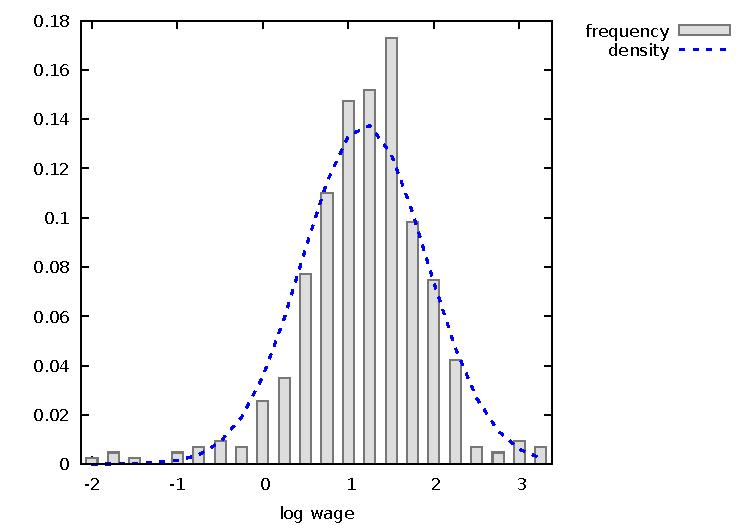
\includegraphics{figures/Mroz-logwage}
  \caption{Output from listing \ref{ex:Mroz-logwage}}
  \label{fig:Mroz-logwage}
\end{figure}

\subsubsection{Example: Plotting Student's $t$ densities}

\begin{script}[htbp]
  \scriptcaption{Plotting $t$ densities for varying degrees of freedom}
  \label{ex:StudentPlot}
\begin{scode}
set verbose off

function string tplot(scalar m)
    return sprintf("stud(x,%d) title \"t(%d)\"", m, m)
end function

matrix dfs = {2, 4, 16}

plot
    literal set xrange [-4.5:4.5]
    literal set yrange [0:0.45]
    literal Binv(p,q) = exp(lgamma(p+q)-lgamma(p)-lgamma(q))
    literal stud(x,m) = Binv(0.5*m,0.5)/sqrt(m)*(1.0+(x*x)/m)**(-0.5*(m+1.0))
    printf "plot %s, %s, %s", tplot(dfs[1]), tplot(dfs[2]), tplot(dfs[3])
end plot --output=display
\end{scode}
\end{script}

The power of the \cmd{printf} statement in a \cmd{plot} block becomes
apparent when used jointly with user-defined functions, as exemplified
in Listing \ref{ex:StudentPlot}, in which we create a plot showing
the density functions of Student's $t$ distribution for three
different settings of the ``degrees of freedom'' parameter (note that
plotting a $t$ density is very easy to do from the GUI: just go to the
\emph{Tools $>$ Distribution graphs} menu).

First we define a user function called \texttt{tplot}, which returns a
string with the ingredients to pass to the gnuplot \texttt{plot}
statement, as a function of a scalar parameter (the degrees of freedom
in our case). Next, this function is used within the \cmd{plot} block
to plot the appropriate density. Note that most of the 
statements to mathematically define the function to plot are
outsourced to gnuplot via the \cmd{literal} command.

The output from the script is shown in Figure \ref{fig:StudentPlot}.

\begin{figure}[htbp]
  \centering
  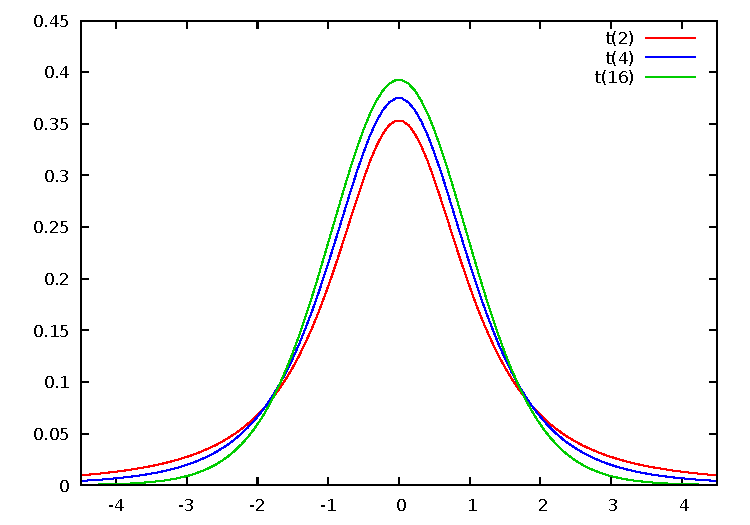
\includegraphics{figures/StudentPlot}
  \caption{Output from listing \ref{ex:StudentPlot}}
  \label{fig:StudentPlot}
\end{figure}


\pagebreak[4]

\section{Boxplots}
\label{sect-boxplots}

These plots (after Tukey and Chambers) display the distribution of a
variable. Its shape depends on a few quantities, defined as follows:

\begin{center}
\begin{tabular}{rl}
  $x_{\mathrm{min}}$ & sample minimum \\
  $Q_1$ & first quartile \\
  $m$ & median \\
  $\bar{x}$ & mean \\
  $Q_3$ & third quartile \\
  $x_{\mathrm{max}}$ & sample maximum\\
  $R = Q_3 - Q_1$ & interquartile range\\
\end{tabular}
\end{center}

The central box encloses the middle 50 percent of the data, i.e.\ goes
from $Q_1$ to $Q_3$; therefore, its height equals $R$.  A line
is drawn across the box at the median $m$ and a ``\texttt{+}'' sign
identifies the mean $\bar{x}$.

The length of the ``whiskers'' depends on the presence of
outliers. The top whisker extends from the top of the box up to a
maximum of 1.5 times the interquartile range, but can be shorter if
the sample maximum is lower than that value; that is, it reaches
$\min[x_{\mathrm{max}}, Q_3 + 1.5 R]$. Observations larger than
$Q_3 + 1.5 R$, if any, are considered outliers and represented
individually via dots.\footnote{To give you an intuitive idea, if a
  variable is normally distributed, the chances of picking an outlier
  by this definition are slightly below 0.7\%.} The bottom whisker
obeys the same logic, with obvious adjustments.
Figure~\ref{fig-boxplot} provides an example of all this by using the
variable \texttt{FAMINC} from the sample dataset \texttt{mroz87}.

\begin{figure}[htbp]
  \begin{flushleft}
    \hspace{1cm}
  \definecolor{c0000ff}{RGB}{0,0,255}
\definecolor{c00cc00}{RGB}{0,204,0}
\begin{tikzpicture}[y=0.80pt, x=0.80pt, yscale=-1.000000, xscale=1.000000, inner sep=0pt, outer sep=0pt]
\begin{scope}[cm={{1.5,0.0,0.0,-1.5,(0.0,336.0)}}]
    \path[draw=black,line join=miter,line cap=rect,miter limit=3.80,line
      width=0.200pt] (38.7500,13.3980) -- (41.8520,13.3980);
    \path[draw=black,line join=miter,line cap=rect,miter limit=3.80,line
      width=0.200pt] (38.7500,228.1990) -- (38.7500,8.5000);
    \path[cm={{1.0,0.0,0.0,-1.0,(29.76698,11.2373)}},fill=black,nonzero rule]
      (0.0000,0.0000) node[above right] (text18) {0};
    \path[draw=black,line join=miter,line cap=rect,miter limit=3.80,line
      width=0.200pt] (38.7500,56.4490) -- (41.8520,56.4490);
    \path[cm={{1.0,0.0,0.0,-1.0,(11.95058,54.28809)}},fill=black,nonzero rule]
      (0.0000,0.0000) node[above right] (text24) {20000};
    \path[draw=black,line join=miter,line cap=rect,miter limit=3.80,line
      width=0.200pt] (38.7500,99.5000) -- (41.8520,99.5000);
    \path[cm={{1.0,0.0,0.0,-1.0,(11.95058,97.33496)}},fill=black,nonzero rule]
      (0.0000,0.0000) node[above right] (text30) {40000};
    \path[draw=black,line join=miter,line cap=rect,miter limit=3.80,line
      width=0.200pt] (38.7500,142.5510) -- (41.8520,142.5510);
    \path[cm={{1.0,0.0,0.0,-1.0,(11.95058,140.38574)}},fill=black,nonzero rule]
      (0.0000,0.0000) node[above right] (text36) {60000};
    \path[draw=black,line join=miter,line cap=rect,miter limit=3.80,line
      width=0.200pt] (38.7500,185.6020) -- (41.8520,185.6020);
    \path[cm={{1.0,0.0,0.0,-1.0,(11.95058,183.43652)}},fill=black,nonzero rule]
      (0.0000,0.0000) node[above right] (text42) {80000};
    \path[draw=black,line join=miter,line cap=rect,miter limit=3.80,line
      width=0.200pt] (38.7500,228.1990) -- (38.7500,8.5000);
    \path[cm={{1.0,0.0,0.0,-1.0,(155,238)}},fill=black,nonzero rule]
      (0.0000,0.0000) node[above right] (text48) {FAMINC};
    \path[draw=c0000ff,line join=miter,line cap=rect,miter limit=3.80,line
      width=0.400pt] (173,16.6480) -- (173,46.6020);
    \path[draw=c0000ff,line join=miter,line cap=rect,miter limit=3.80,line
      width=0.400pt] (173,74.1990) -- (173,114.6020);
    \path[draw=c0000ff,line join=miter,line cap=rect,miter limit=3.80,line
      width=0.400pt] (150,74.1990) -- (196,74.1990) -- (196,46.6010)
      -- (150,46.6010) -- cycle;
    \path[draw=black,line join=miter,line cap=rect,miter limit=3.80,line
      width=0.200pt] (150,58.3520) -- (196,58.3520) -- (150,58.3520);
    \path[draw=c00cc00,line join=miter,line cap=rect,miter limit=3.80,line
      width=0.200pt] (170,63.1020) -- (176,63.1020);
    \path[draw=c00cc00,line join=miter,line cap=rect,miter limit=3.80,line
      width=0.200pt] (173,66.1020) -- (173,60.1020);
    \path[draw=black,fill=black,line join=miter,line cap=rect,miter
      limit=3.80,nonzero rule,line width=0.200pt] (173,115.6480) .. controls
      (173,114.6480) and (172,114.6480) .. (172,115.6480) .. controls
      (172,116.6480) and (173,116.6480) .. (173,115.6480);
    \path[draw=black,fill=black,line join=miter,line cap=rect,miter
      limit=3.80,nonzero rule,line width=0.200pt] (173,117.3980) .. controls
      (173,116.3980) and (172,116.3980) .. (172,117.3980) .. controls
      (172,118.3980) and (173,118.3980) .. (173,117.3980);
    \path[draw=black,fill=black,line join=miter,line cap=rect,miter
      limit=3.80,nonzero rule,line width=0.200pt] (173,118.4490) .. controls
      (173,117.4490) and (172,117.4490) .. (172,118.4490) .. controls
      (172,119.4490) and (173,119.4490) .. (173,118.4490);
    \path[draw=black,fill=black,line join=miter,line cap=rect,miter
      limit=3.80,nonzero rule,line width=0.200pt] (173,120.1990) .. controls
      (173,119.1990) and (172,119.1990) .. (172,120.1990) .. controls
      (172,121.1990) and (173,121.1990) .. (173,120.1990);
    \path[draw=black,fill=black,line join=miter,line cap=rect,miter
      limit=3.80,nonzero rule,line width=0.200pt] (173,121.6990) .. controls
      (173,120.6990) and (172,120.6990) .. (172,121.6990) .. controls
      (172,122.6990) and (173,122.6990) .. (173,121.6990);
    \path[draw=black,fill=black,line join=miter,line cap=rect,miter
      limit=3.80,nonzero rule,line width=0.200pt] (173,122.6480) .. controls
      (173,121.6480) and (172,121.6480) .. (172,122.6480) .. controls
      (172,123.6480) and (173,123.6480) .. (173,122.6480);
    \path[draw=black,fill=black,line join=miter,line cap=rect,miter
      limit=3.80,nonzero rule,line width=0.200pt] (173,123.0000) .. controls
      (173,122.0000) and (172,122.0000) .. (172,123.0000) .. controls
      (172,124.0000) and (173,124.0000) .. (173,123.0000);
    \path[draw=black,fill=black,line join=miter,line cap=rect,miter
      limit=3.80,nonzero rule,line width=0.200pt] (173,123.1990) .. controls
      (173,122.1990) and (172,122.1990) .. (172,123.1990) .. controls
      (172,124.1990) and (173,124.1990) .. (173,123.1990);
    \path[draw=black,fill=black,line join=miter,line cap=rect,miter
      limit=3.80,nonzero rule,line width=0.200pt] (173,123.1990) .. controls
      (173,122.1990) and (172,122.1990) .. (172,123.1990) .. controls
      (172,124.1990) and (173,124.1990) .. (173,123.1990);
    \path[draw=black,fill=black,line join=miter,line cap=rect,miter
      limit=3.80,nonzero rule,line width=0.200pt] (173,123.6020) .. controls
      (173,122.6020) and (172,122.6020) .. (172,123.6020) .. controls
      (172,124.6020) and (173,124.6020) .. (173,123.6020);
    \path[draw=black,fill=black,line join=miter,line cap=rect,miter
      limit=3.80,nonzero rule,line width=0.200pt] (173,126.6480) .. controls
      (173,125.6480) and (172,125.6480) .. (172,126.6480) .. controls
      (172,127.6480) and (173,127.6480) .. (173,126.6480);
    \path[draw=black,fill=black,line join=miter,line cap=rect,miter
      limit=3.80,nonzero rule,line width=0.200pt] (173,126.7500) .. controls
      (173,125.7500) and (172,125.7500) .. (172,126.7500) .. controls
      (172,127.7500) and (173,127.7500) .. (173,126.7500);
    \path[draw=black,fill=black,line join=miter,line cap=rect,miter
      limit=3.80,nonzero rule,line width=0.200pt] (173,131.8010) .. controls
      (173,130.8010) and (172,130.8010) .. (172,131.8010) .. controls
      (172,132.8010) and (173,132.8010) .. (173,131.8010);
    \path[draw=black,fill=black,line join=miter,line cap=rect,miter
      limit=3.80,nonzero rule,line width=0.200pt] (173,133.1020) .. controls
      (173,132.1020) and (172,132.1020) .. (172,133.1020) .. controls
      (172,134.1020) and (173,134.1020) .. (173,133.1020);
    \path[draw=black,fill=black,line join=miter,line cap=rect,miter
      limit=3.80,nonzero rule,line width=0.200pt] (173,134.1480) .. controls
      (173,133.1480) and (172,133.1480) .. (172,134.1480) .. controls
      (172,135.1480) and (173,135.1480) .. (173,134.1480);
    \path[draw=black,fill=black,line join=miter,line cap=rect,miter
      limit=3.80,nonzero rule,line width=0.200pt] (173,136.1020) .. controls
      (173,135.1020) and (172,135.1020) .. (172,136.1020) .. controls
      (172,137.1020) and (173,137.1020) .. (173,136.1020);
    \path[draw=black,fill=black,line join=miter,line cap=rect,miter
      limit=3.80,nonzero rule,line width=0.200pt] (173,136.7500) .. controls
      (173,135.7500) and (172,135.7500) .. (172,136.7500) .. controls
      (172,137.7500) and (173,137.7500) .. (173,136.7500);
    \path[draw=black,fill=black,line join=miter,line cap=rect,miter
      limit=3.80,nonzero rule,line width=0.200pt] (173,139.3520) .. controls
      (173,138.3520) and (172,138.3520) .. (172,139.3520) .. controls
      (172,140.3520) and (173,140.3520) .. (173,139.3520);
    \path[draw=black,fill=black,line join=miter,line cap=rect,miter
      limit=3.80,nonzero rule,line width=0.200pt] (173,147.0000) .. controls
      (173,146.0000) and (172,146.0000) .. (172,147.0000) .. controls
      (172,148.0000) and (173,148.0000) .. (173,147.0000);
    \path[draw=black,fill=black,line join=miter,line cap=rect,miter
      limit=3.80,nonzero rule,line width=0.200pt] (173,147.9490) .. controls
      (173,146.9490) and (172,146.9490) .. (172,147.9490) .. controls
      (172,148.9490) and (173,148.9490) .. (173,147.9490);
    \path[draw=black,fill=black,line join=miter,line cap=rect,miter
      limit=3.80,nonzero rule,line width=0.200pt] (173,149.4490) .. controls
      (173,148.4490) and (172,148.4490) .. (172,149.4490) .. controls
      (172,150.4490) and (173,150.4490) .. (173,149.4490);
    \path[draw=black,fill=black,line join=miter,line cap=rect,miter
      limit=3.80,nonzero rule,line width=0.200pt] (173,150.1020) .. controls
      (173,149.1020) and (172,149.1020) .. (172,150.1020) .. controls
      (172,151.1020) and (173,151.1020) .. (173,150.1020);
    \path[draw=black,fill=black,line join=miter,line cap=rect,miter
      limit=3.80,nonzero rule,line width=0.200pt] (173,156.1480) .. controls
      (173,155.1480) and (172,155.1480) .. (172,156.1480) .. controls
      (172,157.1480) and (173,157.1480) .. (173,156.1480);
    \path[draw=black,fill=black,line join=miter,line cap=rect,miter
      limit=3.80,nonzero rule,line width=0.200pt] (173,159.8520) .. controls
      (173,158.8520) and (172,158.8520) .. (172,159.8520) .. controls
      (172,160.8520) and (173,160.8520) .. (173,159.8520);
    \path[draw=black,fill=black,line join=miter,line cap=rect,miter
      limit=3.80,nonzero rule,line width=0.200pt] (173,171.8520) .. controls
      (173,170.8520) and (172,170.8520) .. (172,171.8520) .. controls
      (172,172.8520) and (173,172.8520) .. (173,171.8520);
    \path[draw=black,fill=black,line join=miter,line cap=rect,miter
      limit=3.80,nonzero rule,line width=0.200pt] (173,179.1480) .. controls
      (173,178.1480) and (172,178.1480) .. (172,179.1480) .. controls
      (172,180.1480) and (173,180.1480) .. (173,179.1480);
    \path[draw=black,fill=black,line join=miter,line cap=rect,miter
      limit=3.80,nonzero rule,line width=0.200pt] (173,185.1020) .. controls
      (173,184.1020) and (172,184.1020) .. (172,185.1020) .. controls
      (172,186.1020) and (173,186.1020) .. (173,185.1020);
    \path[draw=black,fill=black,line join=miter,line cap=rect,miter
      limit=3.80,nonzero rule,line width=0.200pt] (173,202.8520) .. controls
      (173,201.8520) and (172,201.8520) .. (172,202.8520) .. controls
      (172,203.8520) and (173,203.8520) .. (173,202.8520);
    \path[draw=black,fill=black,line join=miter,line cap=rect,miter
      limit=3.80,nonzero rule,line width=0.200pt] (173,208.8520) .. controls
      (173,207.8520) and (172,207.8520) .. (172,208.8520) .. controls
      (172,209.8520) and (173,209.8520) .. (173,208.8520);
    \path[draw=black,fill=black,line join=miter,line cap=rect,miter
      limit=3.80,nonzero rule,line width=0.200pt] (173,209.3980) .. controls
      (173,208.3980) and (172,208.3980) .. (172,209.3980) .. controls
      (172,210.3980) and (173,210.3980) .. (173,209.3980);
    \path[draw=black,fill=black,line join=miter,line cap=rect,miter
      limit=3.80,nonzero rule,line width=0.200pt] (173,220.0510) .. controls
      (173,219.0510) and (172,219.0510) .. (172,220.0510) .. controls
      (172,221.0510) and (173,221.0510) .. (173,220.0510);
    \path[draw=black,line join=miter,line cap=butt,miter limit=4.00,line
      width=0.544pt] (183,64.8980) -- (221,79.1760);
    \begin{scope}[cm={{1.0,0.37854,-0.37854,1.0,(0.0,252.0)}}]
      \path[draw=black,fill=black,line join=miter,line cap=butt,miter limit=4.00,even
        odd rule,line width=0.509pt] (98,-224) -- (100,-226) --
        (93,-224) -- (100,-221) -- cycle;
    \end{scope}
    \path[cm={{1.0,0.0,0.0,-1.0,(224,80)}},fill=black,nonzero rule]
      (0.0000,0.0000) node[above right] (text134) {$\bar{x}$};
    \path[cm={{1.0,0.0,0.0,-1.0,(132.5,76)}},fill=black,nonzero rule]
      (0.0000,0.0000) node[above right] (text142) {$Q_3$};
    \path[cm={{1.0,0.0,0.0,-1.0,(132.5,40)}},fill=black,nonzero rule]
      (0.0000,0.0000) node[above right] (text142) {$Q_1$};
    \path[cm={{1.0,0.0,0.0,-1.0,(132.5,57)}},fill=black,nonzero rule]
      (0.0000,0.0000) node[above right] (text142) {$m$};
    \path[cm={{1.0,0.0,0.0,-1.0,(178,12)}},fill=black,nonzero rule]
      (0.0000,0.0000) node[above right] (text146) {$x_{\mathrm{min}}$};
    \path[cm={{1.0,0.0,0.0,-1.0,(178,218)}},fill=black,nonzero rule]
      (0.0000,0.0000) node[above right] (text146) {$x_{\mathrm{max}}$};
    \path[cm={{1.0,0.0,0.0,-1.0,(110,165)}},fill=black,nonzero rule]
      (0.0000,0.0000) node[above right] (text152) {outliers};
    \path[draw=black,line join=miter,line cap=butt,miter limit=4.00,line
      width=0.626pt] (168,219.8910) .. controls (152,218.0820) and
      (162,185.3050) .. (159,174.6600) .. controls (159,172.9570) and
      (158,170.4340) .. (156,169.8520) .. controls (154,169.4100) and
      (153,168.6050) .. (151,168.0270) .. controls (153,167.4300) and
      (155,166.6450) .. (156,166.2070) .. controls (158,165.6250) and
      (160,163.0980) .. (160,161.3980) .. controls (162,150.7500) and
      (152,117.9770) .. (168,116.1680);
\end{scope}

\end{tikzpicture}

%%% Local Variables:
%%% mode: latex
%%% TeX-master: "../tex/gretl-guide"
%%% End:

  \end{flushleft}
  \caption{Sample boxplot}
  \label{fig-boxplot}
\end{figure}

In the case of boxplots with confidence intervals, dotted lines show
the limits of an approximate 90 percent confidence interval for the
median.  This is obtained by the bootstrap method, which can take a
while if the data series is very long. For details on constructing
boxplots, see the entry for \cmd{boxplot} in the \GCR\, or use the
\textsf{Help} button that appears when you select one of the boxplot
items under the menu item ``View, Graph specified vars'' in the main
gretl window.

\subsection{Factorized boxplots}

A nice feature which is quite useful for data visualization is the
conditional, or factorized boxplot.  This type of plot allows you to
examine the distribution of a variable conditional on the value of
some discrete factor.

As an example, we'll use one of the datasets supplied with
gretl, that is \cmd{rac3d}, which contains an example taken from
\cite{cameron-trivedi13} on the health conditions of 5190 people. The
script below compares the unconditional (marginal) distribution of the
number of illnesses in the past 2 weeks with the distribution of the
same variable, conditional on age classes.

\begin{scode}
open rac3d.gdt
# unconditional boxplot
boxplot ILLNESS --output=display
# create a discrete variable for age class: 
# 0 = below 20, 1 = between 20 and 39, etc
series age_class = floor(AGE/0.2)
# conditional boxplot
boxplot ILLNESS age_class --factorized --output=display
\end{scode}

After running the code above, you should see two graphs similar to
Figure \ref{fig:fact-boxplots}. By comparing the marginal plot to
the factorized one, the effect of age on the mean number of illnesses
is quite evident: by joining the green crosses you get what is
technically known as the conditional mean function, or regression
function if you prefer.

\begin{figure}[htbp]
  \centering
  \begin{tabular}{cc}
    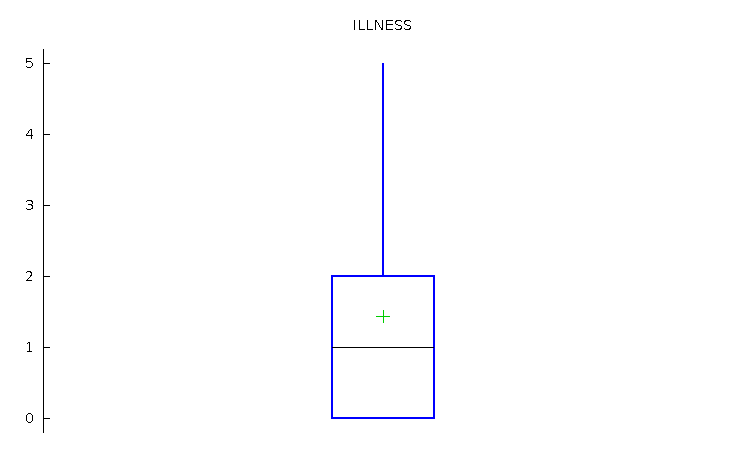
\includegraphics[width=0.475\textwidth]{figures/uboxplot} & 
    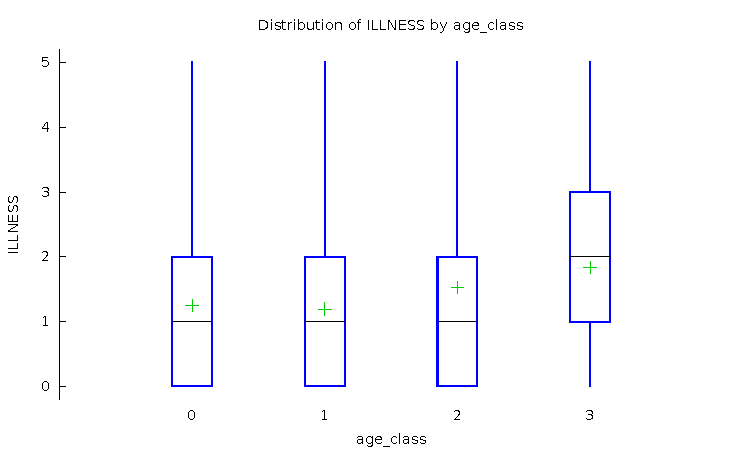
\includegraphics[width=0.475\textwidth]{figures/fboxplot}
  \end{tabular}
  \caption{Conditional and unconditional distribution of illnesses}
  \label{fig:fact-boxplots}
\end{figure}

%%% Local Variables: 
%%% mode: latex
%%% TeX-master: "gretl-guide"
%%% End: 

